% Options for packages loaded elsewhere
\PassOptionsToPackage{unicode}{hyperref}
\PassOptionsToPackage{hyphens}{url}
%
\documentclass[
  10pt,
  ignorenonframetext,
]{beamer}
\usepackage{pgfpages}
\setbeamertemplate{caption}[numbered]
\setbeamertemplate{caption label separator}{: }
\setbeamercolor{caption name}{fg=normal text.fg}
\beamertemplatenavigationsymbolsempty
% Prevent slide breaks in the middle of a paragraph
\widowpenalties 1 10000
\raggedbottom
\setbeamertemplate{part page}{
  \centering
  \begin{beamercolorbox}[sep=16pt,center]{part title}
    \usebeamerfont{part title}\insertpart\par
  \end{beamercolorbox}
}
\setbeamertemplate{section page}{
  \centering
  \begin{beamercolorbox}[sep=12pt,center]{part title}
    \usebeamerfont{section title}\insertsection\par
  \end{beamercolorbox}
}
\setbeamertemplate{subsection page}{
  \centering
  \begin{beamercolorbox}[sep=8pt,center]{part title}
    \usebeamerfont{subsection title}\insertsubsection\par
  \end{beamercolorbox}
}
\AtBeginPart{
  \frame{\partpage}
}
\AtBeginSection{
  \ifbibliography
  \else
    \frame{\sectionpage}
  \fi
}
\AtBeginSubsection{
  \frame{\subsectionpage}
}
\usepackage{amsmath,amssymb}
\usepackage{iftex}
\ifPDFTeX
  \usepackage[T1]{fontenc}
  \usepackage[utf8]{inputenc}
  \usepackage{textcomp} % provide euro and other symbols
\else % if luatex or xetex
  \usepackage{unicode-math} % this also loads fontspec
  \defaultfontfeatures{Scale=MatchLowercase}
  \defaultfontfeatures[\rmfamily]{Ligatures=TeX,Scale=1}
\fi
\usepackage{lmodern}
\usetheme[]{AnnArbor}
\usecolortheme{dolphin}
\usefonttheme{structurebold}
\ifPDFTeX\else
  % xetex/luatex font selection
\fi
% Use upquote if available, for straight quotes in verbatim environments
\IfFileExists{upquote.sty}{\usepackage{upquote}}{}
\IfFileExists{microtype.sty}{% use microtype if available
  \usepackage[]{microtype}
  \UseMicrotypeSet[protrusion]{basicmath} % disable protrusion for tt fonts
}{}
\makeatletter
\@ifundefined{KOMAClassName}{% if non-KOMA class
  \IfFileExists{parskip.sty}{%
    \usepackage{parskip}
  }{% else
    \setlength{\parindent}{0pt}
    \setlength{\parskip}{6pt plus 2pt minus 1pt}}
}{% if KOMA class
  \KOMAoptions{parskip=half}}
\makeatother
\usepackage{xcolor}
\newif\ifbibliography
\usepackage{graphicx}
\makeatletter
\def\maxwidth{\ifdim\Gin@nat@width>\linewidth\linewidth\else\Gin@nat@width\fi}
\def\maxheight{\ifdim\Gin@nat@height>\textheight\textheight\else\Gin@nat@height\fi}
\makeatother
% Scale images if necessary, so that they will not overflow the page
% margins by default, and it is still possible to overwrite the defaults
% using explicit options in \includegraphics[width, height, ...]{}
\setkeys{Gin}{width=\maxwidth,height=\maxheight,keepaspectratio}
% Set default figure placement to htbp
\makeatletter
\def\fps@figure{htbp}
\makeatother
\setlength{\emergencystretch}{3em} % prevent overfull lines
\providecommand{\tightlist}{%
  \setlength{\itemsep}{0pt}\setlength{\parskip}{0pt}}
\setcounter{secnumdepth}{-\maxdimen} % remove section numbering
\ifLuaTeX
  \usepackage{selnolig}  % disable illegal ligatures
\fi
\usepackage{bookmark}
\IfFileExists{xurl.sty}{\usepackage{xurl}}{} % add URL line breaks if available
\urlstyle{same}
\hypersetup{
  pdftitle={Variograma},
  pdfauthor={Sergio Nava},
  hidelinks,
  pdfcreator={LaTeX via pandoc}}

\title{Variograma}
\author{Sergio Nava}
\date{24/3/2023}

\begin{document}
\frame{\titlepage}

\section{Introducción al
Semivariograma}\label{introducciuxf3n-al-semivariograma}

\begin{frame}{Introducción al Semivariograma}
\begin{itemize}
\tightlist
\item
  El \textbf{semivariograma} es una herramienta fundamental en
  \textbf{geoestadística} para medir la dependencia espacial de un
  conjunto de datos.
\item
  Fue inicialmente utilizado para predecir la presencia de yacimientos
  de oro y petróleo en Sudáfrica.
\item
  La primera ley de la geografía, formulada por \textbf{Waldo Tobler} en
  1970, establece que ``todas las cosas están relacionadas entre sí,
  pero las cosas más próximas en el espacio tienen una relación mayor
  que las distantes``.
\item
  Se utiliza para describir cómo varía la similitud entre puntos en
  función de la distancia que los separa.
\item
  Su análisis es esencial para la interpolación mediante Kriging y otros
  métodos espaciales.
\end{itemize}
\end{frame}

\begin{frame}
\begin{figure}
    \centering
    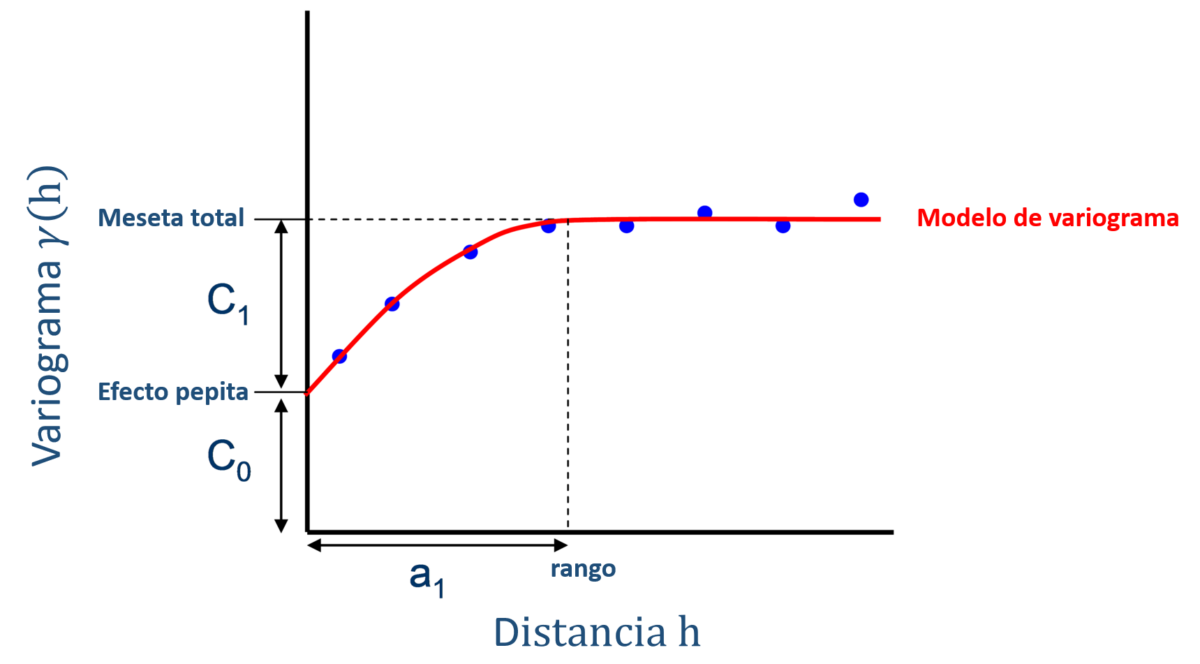
\includegraphics[width=0.6\textwidth]{./imagenes/figura1.png}
    \caption{Ejemplo de un semivariograma empírico y su ajuste.}
\end{figure}
\end{frame}

\section{Diferencia entre Variograma y
Semivariograma}\label{diferencia-entre-variograma-y-semivariograma}

\begin{frame}{Diferencia entre Variograma y Semivariograma}
\begin{itemize}
\item
  \textbf{Variograma:} Representa la varianza de las diferencias entre
  puntos separados por una distancia específica. Se calcula como:

  \begin{equation}
  2\gamma(h) =  \text{Var}[Z(s_i) - Z(s_i + h)]
  \end{equation}
\item
  \textbf{Semivariograma:} Es la mitad del variograma y se usa con mayor
  frecuencia en geoestadística debido a su estabilidad matemática:

  \begin{equation}
  \gamma(h) = \frac{1}{2}   \text{Var}[Z(s_i) - Z(s_i + h)]
  \end{equation}
\item
  El semivariograma es más comúnmente utilizado en aplicaciones
  prácticas ya que facilita el modelado y la interpolación espacial.
\end{itemize}
\end{frame}

\section{Parámetros Clave del
Semivariograma}\label{paruxe1metros-clave-del-semivariograma}

\begin{frame}{Parámetros Clave del Semivariograma}
\begin{itemize} \footnotesize 
   \item \textbf{Pepita o Nugget } $C_0$: Representa una discontinuidad puntual del semivariograma en el origen. Puede deberse a errores de medición o a la escala de la variable observada. 
   \item \textbf{Meseta, Umbral o Sill} $C_1$: Es la varianza de los datos. Se denota por $C_0$  o por $C_0 + C_1$ cuando la pepita es diferente de cero. Si el ruido espacial domina sobre la correlación, las predicciones pueden ser poco precisas.
   \item \textbf{Rango o Range} : Es la distancia hasta la cual existe correlación entre los datos. Un rango pequeño sugiere independencia espacial entre los puntos, mientras que un rango más grande indica una estructura espacial más fuerte. 
\end{itemize}

\begin{figure}
    \centering
    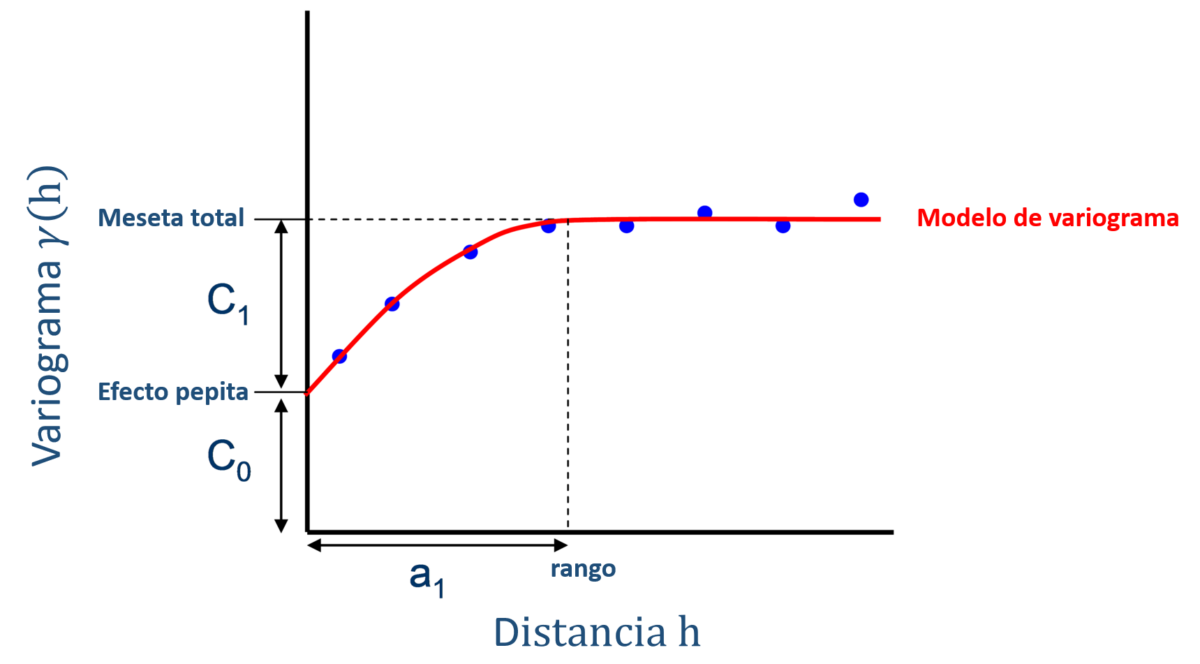
\includegraphics[width=0.5\textwidth]{./imagenes/figura1.png}
    \caption{Ilustración de los parámetros clave del semivariograma.}
\end{figure}
\end{frame}

\begin{frame}
\begin{figure}
\centering
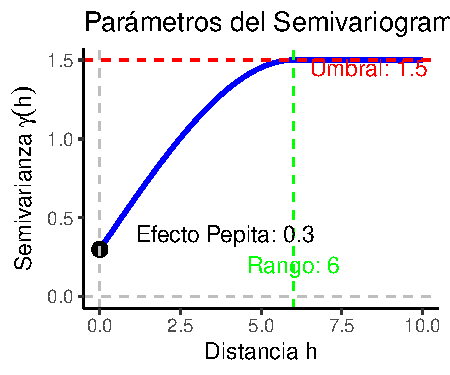
\includegraphics{imagenes/unnamed-chunk-1-1.pdf}
\caption{Visualización de los parámetros clave del semivariograma. Se
ilustran el umbral (línea roja discontinua), que representa la varianza
total del proceso; el rango (línea verde discontinua), que indica la
distancia a la que el semivariograma alcanza el umbral; y el efecto
pepita (punto negro), que refleja la variabilidad no explicada a escala
muy pequeña.}
\end{figure}
\end{frame}

\section{Variograma Cloud}\label{variograma-cloud}

\begin{frame}{Variograma Cloud}
\begin{itemize}
\tightlist
\item
  El \textbf{variograma cloud} es una herramienta exploratoria en
  geoestadística que permite visualizar la dispersión de los valores del
  semivariograma para cada par de puntos.
\item
  En lugar de promediar los valores de semivarianza por intervalos de
  distancia, muestra cada punto individualmente, lo que ayuda a detectar
  anomalías o patrones en los datos espaciales.
\item
  Se utiliza para evaluar la presencia de valores atípicos y verificar
  la estructura de dependencia espacial en los datos.
\end{itemize}

\begin{figure}
\centering
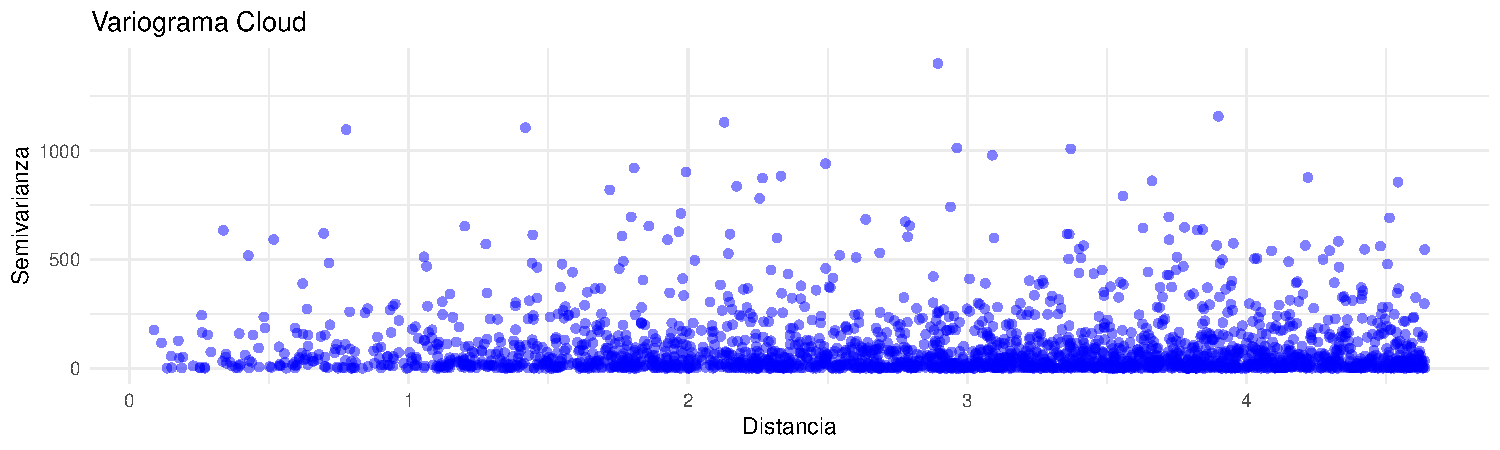
\includegraphics{imagenes/unnamed-chunk-2-1.pdf}
\caption{Ejemplo de Variograma Cloud}
\end{figure}
\end{frame}

\section{Relación entre el Semivariograma y la
Correlación}\label{relaciuxf3n-entre-el-semivariograma-y-la-correlaciuxf3n}

\begin{frame}{Relación entre el Semivariograma y la Correlación}
\begin{itemize}
\item
  La \textbf{función de correlación} describe la similitud entre valores
  de una variable en diferentes ubicaciones espaciales.
\item
  Existe una relación matemática entre el semivariograma y la función de
  correlación:

  \begin{equation}
  \rho(h) = 1 - \frac{\gamma(h)}{\gamma(\infty)}
  \end{equation}

  donde:

  \begin{itemize}
  \tightlist
  \item
    \(\rho(h)\) es la función de correlación.
  \item
    \(\gamma(h)\) es el semivariograma.
  \item
    \(\gamma(\infty)\) es el umbral del semivariograma.
  \end{itemize}
\item
  A medida que la distancia \(h\) aumenta, la correlación decrece y el
  semivariograma se estabiliza en su umbral.
\item
  En un proceso espacial estacionario, la correlación decrece con la
  distancia de manera similar al crecimiento del semivariograma.
\end{itemize}
\end{frame}

\section{Definición del
Semivariograma}\label{definiciuxf3n-del-semivariograma}

\begin{frame}{Definición del Semivariograma}
El semivariograma se define matemáticamente como:

\begin{equation}
\gamma(h) = \frac{1}{2N(h)} \sum_{i=1}^{N(h)} [Z(s_i) - Z(s_i + h)]^2
\end{equation}

Donde:

\begin{itemize}
\tightlist
\item
  \(\gamma(h)\) es la semivarianza para una distancia \(h\).
\item
  \(N(h)\) es el número de pares de puntos separados por la distancia
  \(h\).
\item
  \(Z(s_i)\) es el valor de la variable en la ubicación \(s_i\).
\end{itemize}
\end{frame}

\section{Tipos de Semivariogramas}\label{tipos-de-semivariogramas}

\begin{frame}{Semivariograma Empírico}
\phantomsection\label{semivariograma-empuxedrico}
\begin{itemize}
\tightlist
\item
  Se calcula a partir de datos observados.
\item
  Representa la variabilidad espacial en diferentes escalas.
\end{itemize}
\end{frame}

\begin{frame}{Semivariograma Teórico}
\phantomsection\label{semivariograma-teuxf3rico}
\begin{itemize}
\tightlist
\item
  Se modela mediante funciones matemáticas.
\item
  Modelos más comunes:
\end{itemize}

\begin{figure}
\centering
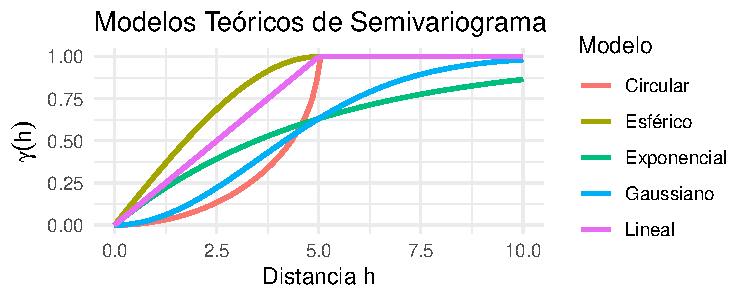
\includegraphics{imagenes/unnamed-chunk-3-1.pdf}
\caption{Ejemplo de diferentes modelos teóricos de semivariograma.}
\end{figure}
\end{frame}

\begin{frame}
\begin{center}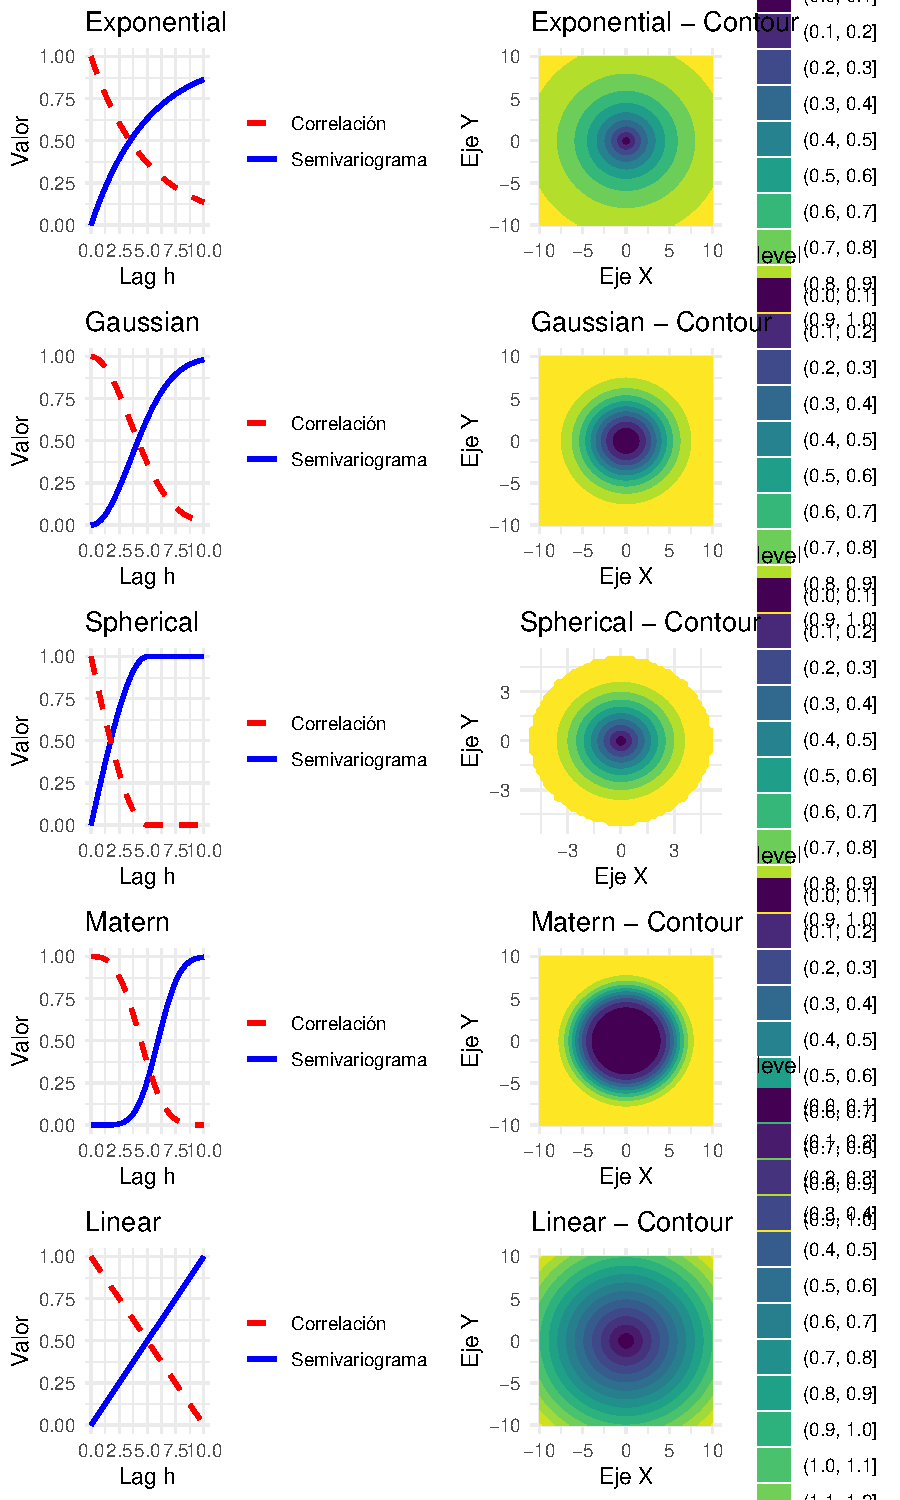
\includegraphics{imagenes/unnamed-chunk-4-1} \end{center}
\end{frame}

\section{Procesos Estacionarios y No
Estacionarios}\label{procesos-estacionarios-y-no-estacionarios}

\begin{frame}{Procesos Estacionarios y No Estacionarios}
\begin{itemize}
\tightlist
\item
  \textbf{Estacionarios:} La media y la varianza son constantes a través
  del espacio.
\item
  \textbf{No estacionarios:} Presentan tendencias o patrones en los
  datos espaciales.
\end{itemize}

\begin{figure}
    \centering
    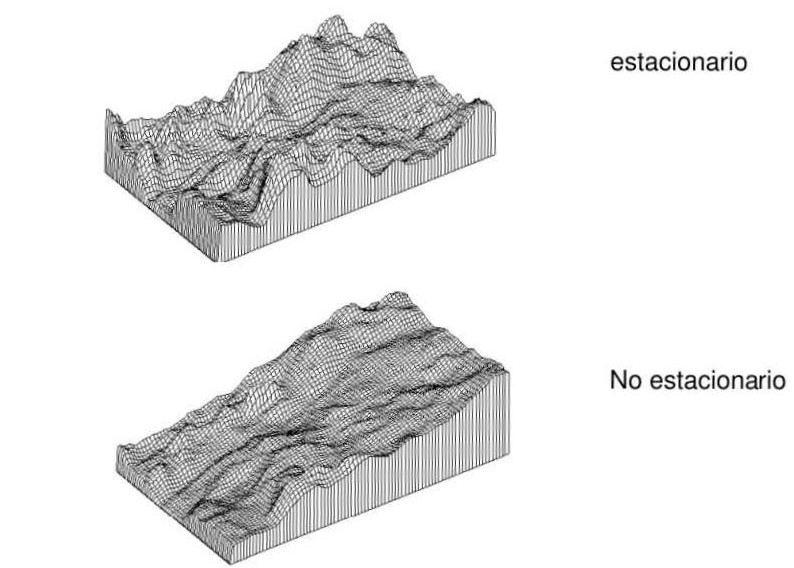
\includegraphics[width=0.6\textwidth]{./imagenes/figura3.jpg}
    \caption{Ejemplo de procesos estacionarios y no estacionarios.}
\end{figure}
\end{frame}

\begin{frame}
\begin{itemize}
\tightlist
\item
  \textbf{Estacionarios:} La media y la varianza son constantes a través
  del espacio.
\end{itemize}

\begin{figure}
    \centering
    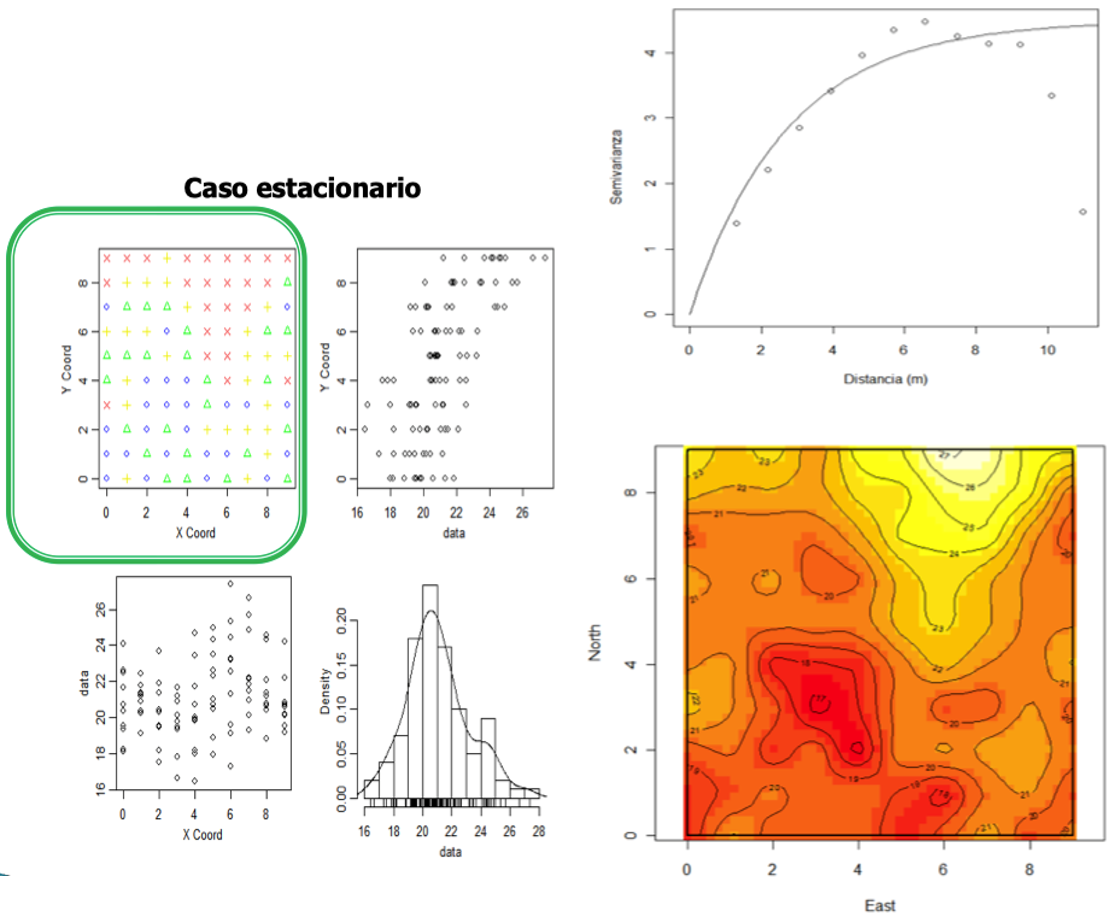
\includegraphics[width=0.6\textwidth]{./imagenes/figura3a.png}
    \caption{Ejemplo de un proceso estacionario.}
\end{figure}
\end{frame}

\begin{frame}
\begin{itemize}
\tightlist
\item
  \textbf{No estacionarios:} Presentan tendencias o patrones en los
  datos espaciales.
\end{itemize}

\begin{figure}
    \centering
    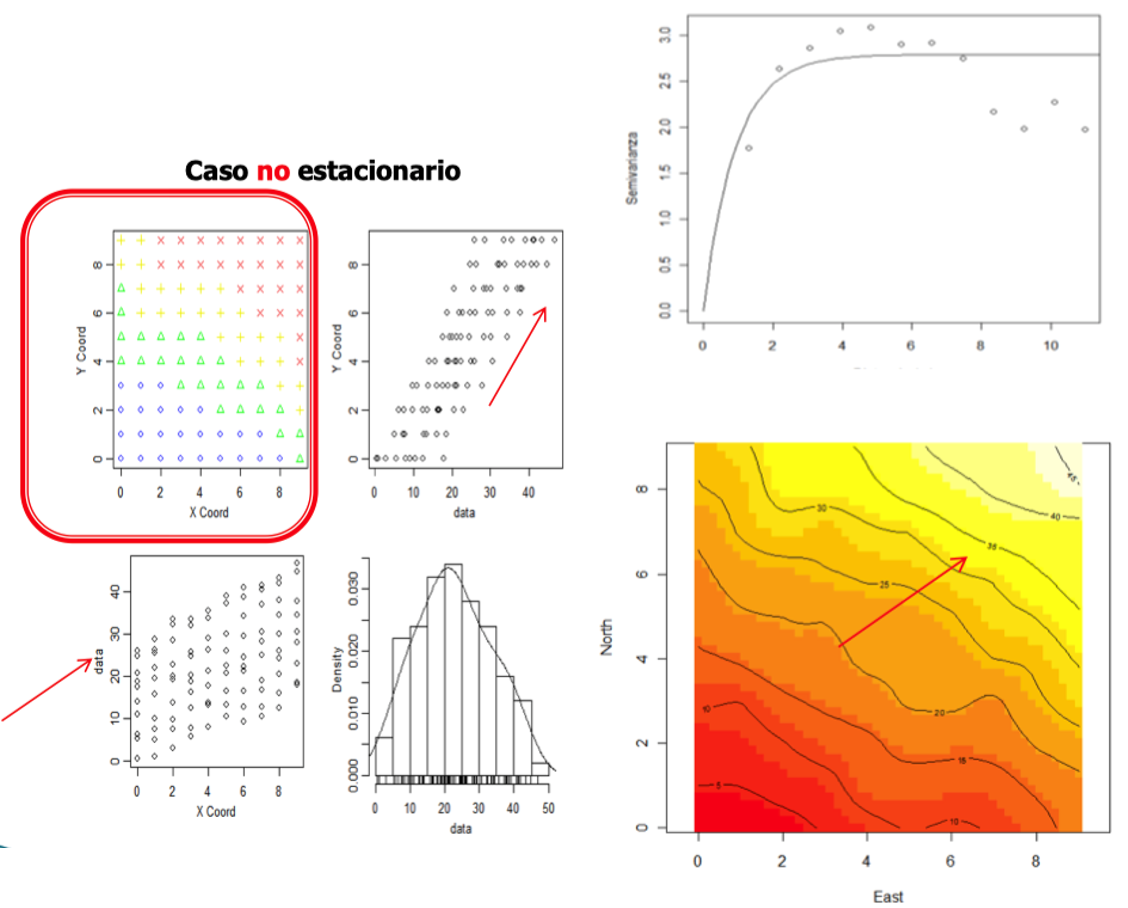
\includegraphics[width=0.6\textwidth]{./imagenes/figura3b.png}
    \caption{Ejemplo de un proceso no estacionario.}
\end{figure}
\end{frame}

\section{Análisis estructural
espacial}\label{anuxe1lisis-estructural-espacial}

\begin{frame}{Análisis estructural espacial}
\begin{itemize}
\tightlist
\item
  Determinar la estructura de relación entre los datos mediante el
  semivariograma.
\item
  Si el semivariograma varía en diferentes direcciones, indica
  \textbf{anisotropía}.
\item
  Si solo depende de la distancia, se considera \textbf{isotrópico}.
\end{itemize}
\end{frame}

\begin{frame}
\begin{figure}

{\centering 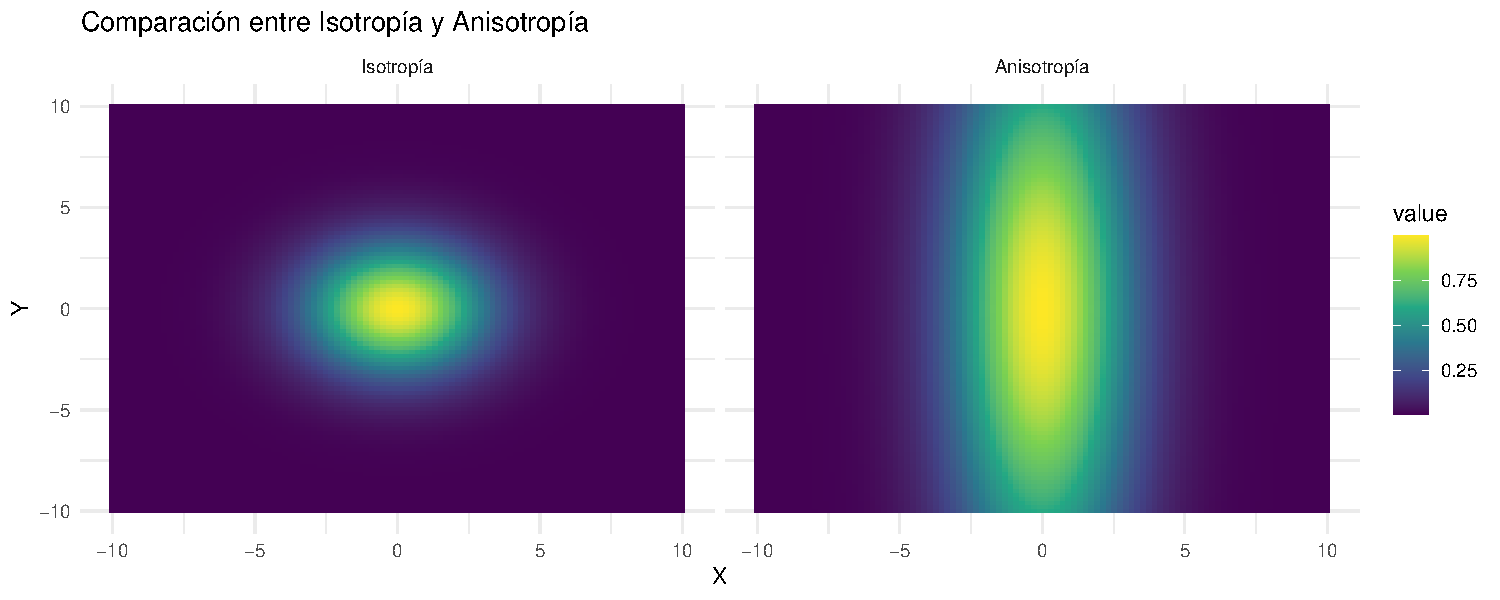
\includegraphics{imagenes/anisotropia-1} 

}

\caption{Visualización comparativa de isotropía y anisotropía en datos espaciales. La figura muestra cómo la variabilidad se distribuye de manera uniforme en todas las direcciones en un proceso isotrópico, mientras que en un proceso anisotrópico la variabilidad es distinta según la dirección, evidenciando mayor dependencia espacial en un eje específico.}\label{fig:anisotropia}
\end{figure}
\end{frame}

\begin{frame}
\begin{block}{Anisotropía}
\phantomsection\label{anisotropuxeda}
\begin{figure}

{\centering 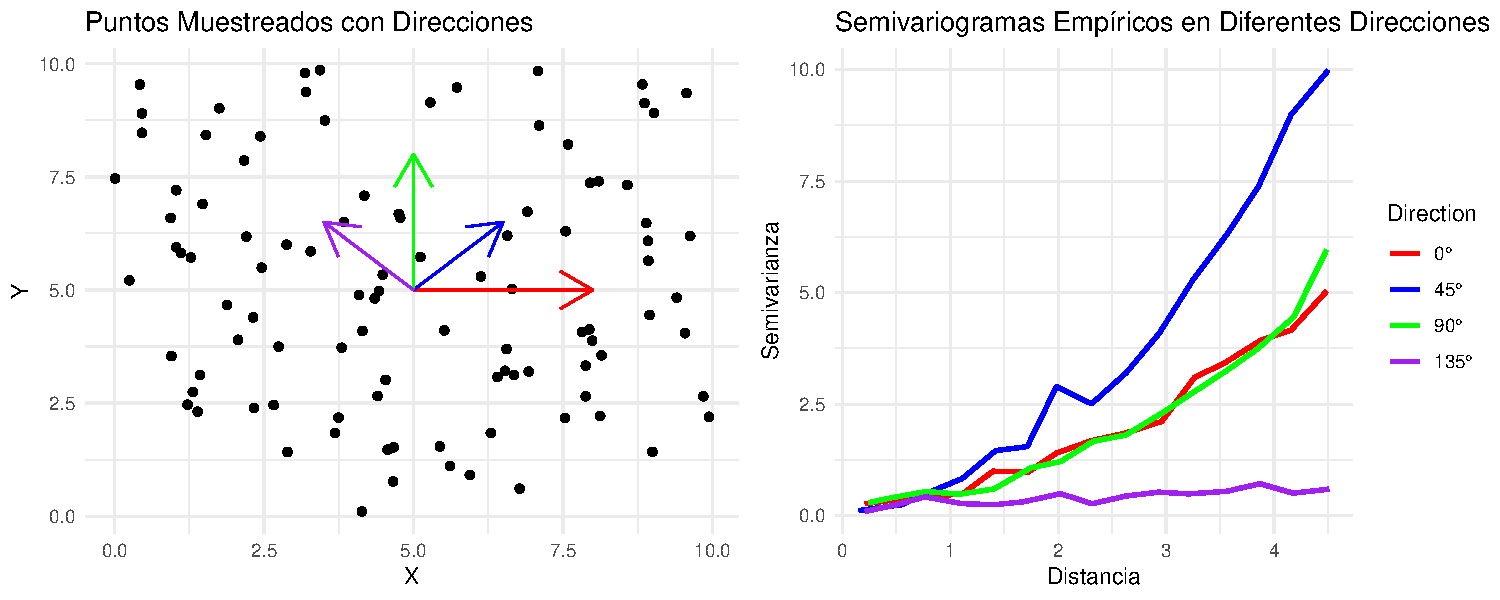
\includegraphics{imagenes/unnamed-chunk-5-1} 

}

\caption{Comparación de semivariogramas empíricos en distintas direcciones para detectar anisotropía en los datos espaciales. A la izquierda, se muestran los puntos muestreados con las direcciones de análisis. A la derecha, los semivariogramas estimados en 0°, 45°, 90° y 135° revelan variaciones en la estructura espacial, evidenciando la presencia de anisotropía si los patrones difieren entre direcciones.}\label{fig:unnamed-chunk-5}
\end{figure}
\end{block}
\end{frame}

\begin{frame}
\begin{block}{Isotropía}
\phantomsection\label{isotropuxeda}
\begin{itemize} \footnotesize
    \item En un proceso \textbf{isotrópico}, la variabilidad espacial es la misma en todas las direcciones.
    \item Se espera que los semivariogramas calculados en distintas direcciones sean similares.
    \item En la siguiente figura se muestra la comparación de semivariogramas empíricos en diferentes direcciones para un proceso isotrópico.
\end{itemize}

\begin{figure}

{\centering 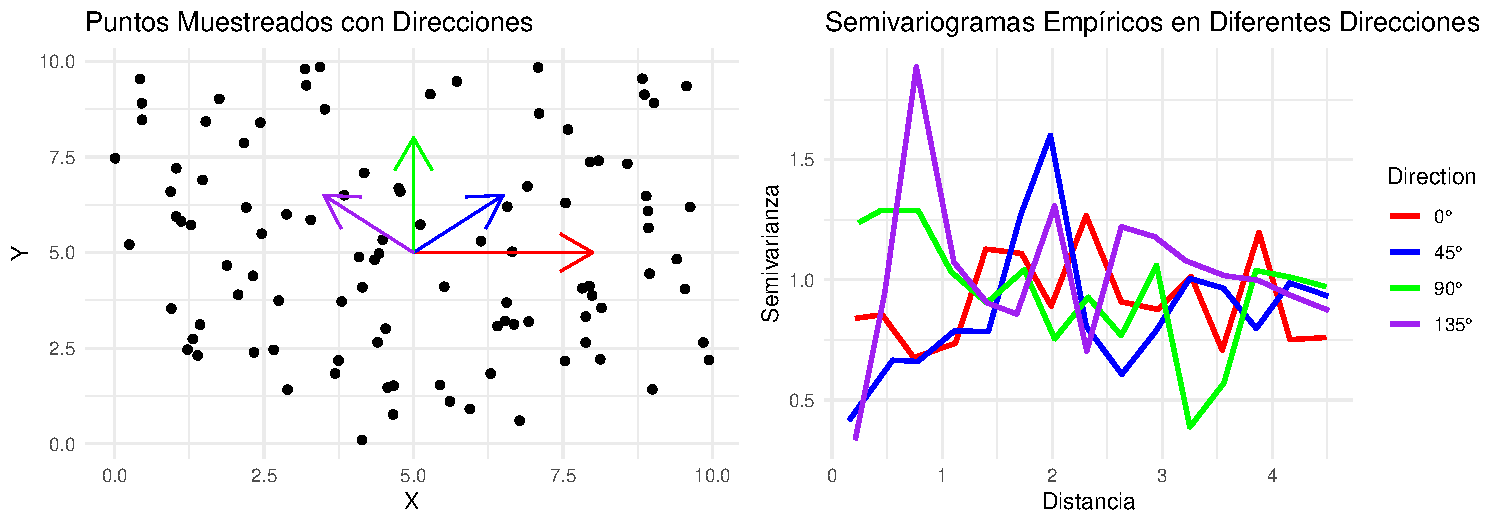
\includegraphics{imagenes/unnamed-chunk-6-1} 

}

\caption{Comparación de semivariogramas empíricos en distintas direcciones para evaluar isotropía en los datos espaciales. A la izquierda, se muestran los puntos muestreados con las direcciones de análisis. A la derecha, los semivariogramas estimados en 0°, 45°, 90° y 135° presentan patrones similares en todas las direcciones, lo que indica que la variabilidad espacial es independiente de la orientación.}\label{fig:unnamed-chunk-6}
\end{figure}
\end{block}
\end{frame}

\begin{frame}
\begin{figure}
    \centering
    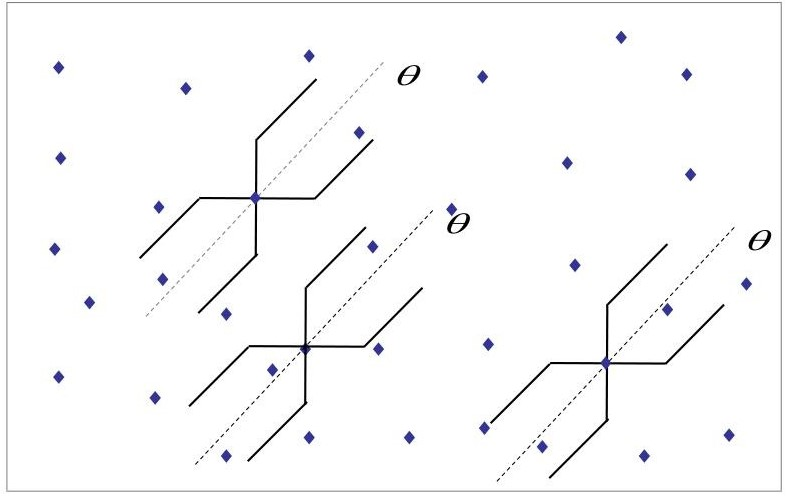
\includegraphics[width=0.6\textwidth]{./imagenes/variograma-dir1.jpg}
    \caption{Cálculo del variograma en dirección $\theta$.}
\end{figure}
\end{frame}

\section{Gráfica del Semivariograma en
R}\label{gruxe1fica-del-semivariograma-en-r}

\begin{frame}{Gráfica del Semivariograma en R}
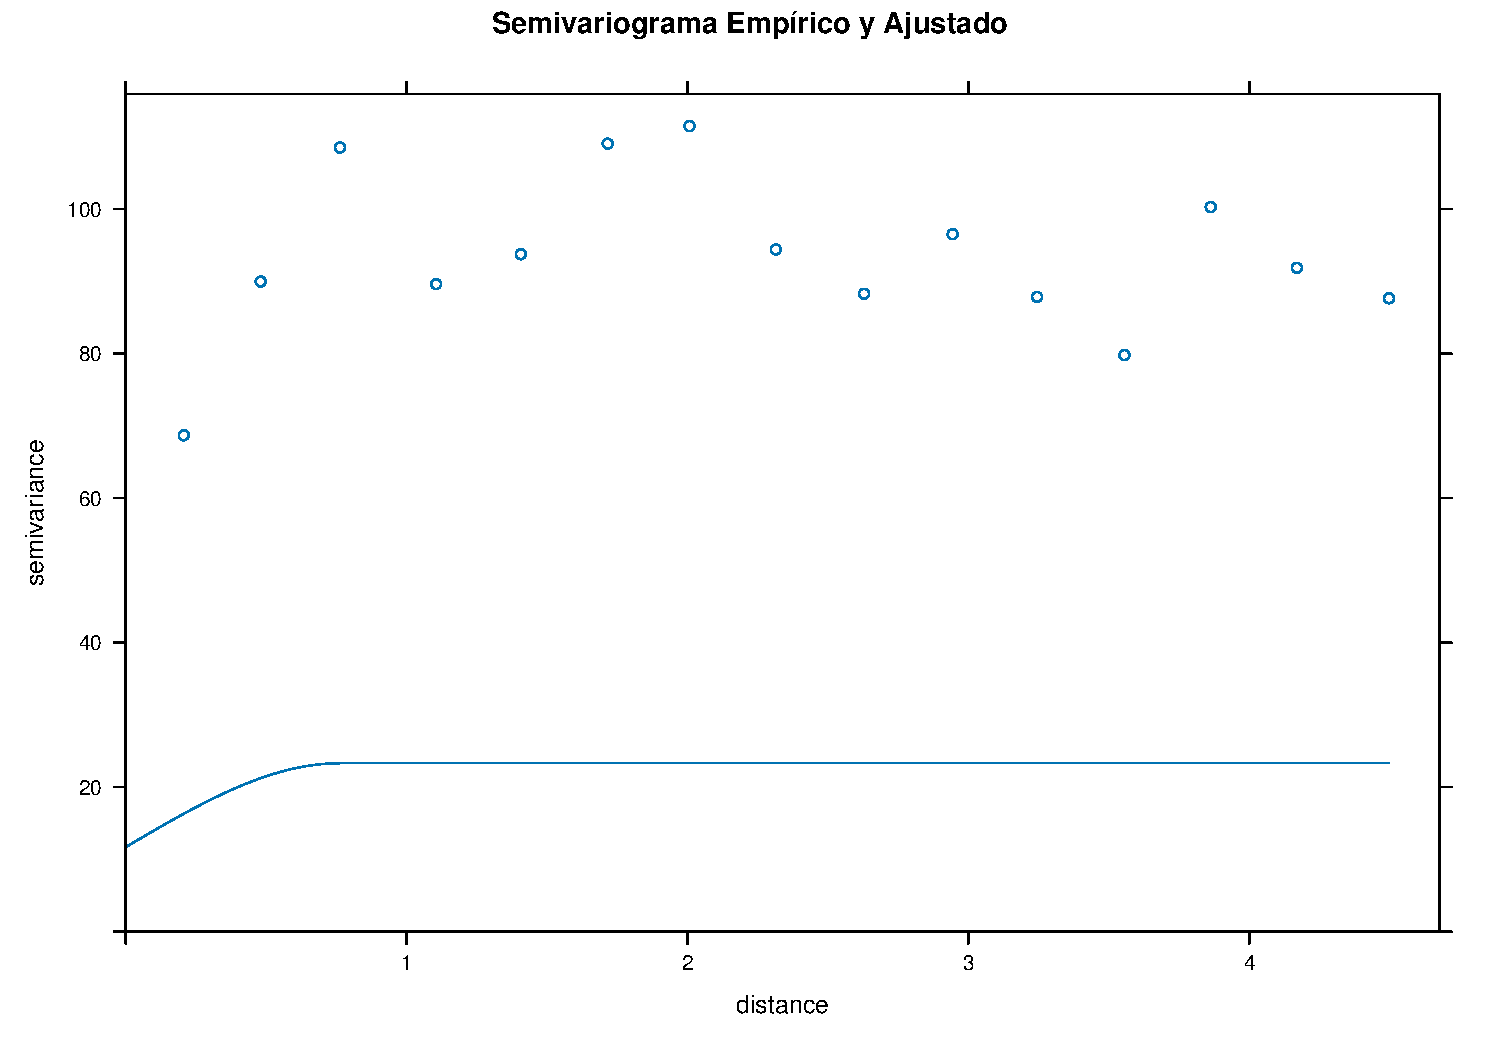
\includegraphics{imagenes/Semivariograma_en_R-1.pdf}
\end{frame}

\section{Conclusión}\label{conclusiuxf3n}

\begin{frame}{Conclusión}
\begin{itemize}
\tightlist
\item
  El semivariograma es una herramienta clave en \textbf{geoestadística}.
\item
  Permite caracterizar la estructura espacial de los datos y mejorar los
  modelos de predicción mediante \textbf{Kriging}.
\item
  Su correcta implementación mejora la precisión de los análisis
  espaciales y sus aplicaciones prácticas en diversos campos como la
  geología, ecología y salud pública.
\end{itemize}
\end{frame}

\end{document}
